%%%%%%%%%%%%%%%%%%%%%%%%%%%%%%%%%%%%%%%%%
% Stylish Article
% LaTeX Template
% Version 2.2 (2020-10-22)
%
% This template has been downloaded from:
% http://www.LaTeXTemplates.com
%
% Original author:
% Mathias Legrand (legrand.mathias@gmail.com) 
% With extensive modifications by:
% Vel (vel@latextemplates.com)
%
% License:
% CC BY-NC-SA 3.0 (http://creativecommons.org/licenses/by-nc-sa/3.0/)
%
%%%%%%%%%%%%%%%%%%%%%%%%%%%%%%%%%%%%%%%%%

%----------------------------------------------------------------------------------------
%	PACKAGES AND OTHER DOCUMENT CONFIGURATIONS
%----------------------------------------------------------------------------------------

\documentclass[fleqn,10pt]{SelfArx} % Document font size and equations flushed left
\usepackage[x11names]{xcolor}
\usepackage[left=1.5cm,right=1.5cm,top=1.5cm,bottom=2cm]{geometry}
\usepackage{newtxtext,newtxmath}
\usepackage{amsmath}
\usepackage{bm}
\usepackage{float}
\usepackage{multicol,multirow}
\usepackage{tabularx}
\usepackage[inline,shortlabels]{enumitem}
\usepackage{cancel}
\usepackage{venndiagram}

%----------------------------------------------------------------------------------------
%	COLUMNS
%----------------------------------------------------------------------------------------

\setlength{\columnsep}{0.55cm} % Distance between the two columns of text
\setlength{\fboxrule}{0.75pt} % Width of the border around the abstract

%----------------------------------------------------------------------------------------
%	COLORS
%----------------------------------------------------------------------------------------

\definecolor{color1}{RGB}{0,0,90} % Color of the article title and sections
\definecolor{color2}{RGB}{0,20,20} % Color of the boxes behind the abstract and headings

%----------------------------------------------------------------------------------------
%	HYPERLINKS
%----------------------------------------------------------------------------------------

\hypersetup{
	hidelinks,
	colorlinks,
	breaklinks=true,
	urlcolor=color2,
	citecolor=color1,
	linkcolor=color1,
	bookmarksopen=false,
	pdftitle={Title},
	pdfauthor={Author},
}

%----------------------------------------------------------------------------------------
%	ARTICLE INFORMATION
%----------------------------------------------------------------------------------------

\JournalInfo{ENGG1300C, Gp. C9, 2024/25-Spring} % Journal information
\Archive{Final Report for Practical Work} % Additional notes (e.g. copyright, DOI, review/research article)

\PaperTitle{Final Report for Practical Work of the Course ENGG1300 of Group C9} % Article title

\Authors{
	Author A\textsuperscript{1},
	Author B\textsuperscript{2},
	Author C\textsuperscript{3},
	Author D\textsuperscript{4},
	Zhan Ho Jacob Shing\textsuperscript{5},
	Author F\textsuperscript{6},
	Author G\textsuperscript{7}
} % Authors
\affiliation{\textbf{*Authors are listed in alphabetical order by surname.}}
\affiliation{\textsuperscript{1}Bachelor of Engineering (\textit{BEng}), 3036******} % Author affiliation
\affiliation{\textsuperscript{2}Bachelor of Engineering (\textit{BEng}), 3036******} % Author affiliation
\affiliation{\textsuperscript{3}Bachelor of Engineering (\textit{BEng}), 3036******} % Author affiliation
\affiliation{\textsuperscript{4}Bachelor of Engineering (\textit{BEng}), 3036******\columnbreak\par} % Author affiliation
\affiliation{\textsuperscript{5}Bachelor of Engineering (\textit{BEng}), 3036******} % Author affiliation
\affiliation{\textsuperscript{6}Bachelor of Engineering (\textit{BEng}), 3036******} % Author affiliation
\affiliation{\textsuperscript{7}Bachelor of Engineering (\textit{BEng}), 3036******} % Author affiliation

\Keywords{} % Keywords - if you don't want any simply remove all the text between the curly brackets
\newcommand{\keywordname}{Keywords} % Defines the keywords heading name

%----------------------------------------------------------------------------------------
%	ABSTRACT
%----------------------------------------------------------------------------------------

\Abstract{
	This report aims to summarise the practical work done for the course ENGG1300 -- Fundamental Mechanics in the second semester of the academic year 2024/25 by Group C9.
	This report introduces the problem presented to the group in the practical work,
	the process of drafting and verifying, and the methodology of the solution,
	the theorems and principles on which the solution is based,
	the results and quantitative analysis of the results,
	and the conclusion and reflection on the practical work.
}

%----------------------------------------------------------------------------------------

\begin{document}

\maketitle % Output the title and abstract box

\tableofcontents % Output the contents section

\thispagestyle{empty} % Removes page numbering from the first page

%----------------------------------------------------------------------------------------
%	ARTICLE CONTENTS
%----------------------------------------------------------------------------------------

\section*{Introduction}
\addcontentsline{toc}{section}{Introduction} % Adds this section to the table of contents

The group was presented a problem to design and realise a structure using only ordinary
	newspapers and transparent plastic adhesive tapes. The problem further specified that
	the said structure shall observe the following conditions:

\begin{enumerate}[noitemsep]
	\item The structure must stand on its own without any external support.
	\item The height of the structure must be between $780$ mm and $800$ mm.
	\item The structure must not weight more than $1$ kg.
	\item The structure shall be able to bear at least $500$ N of load without excessive
		deformation when being compressed by two wooden plates of $480$ mm $\times$ $480$ mm
		$\times$ $10$ mm.
\end{enumerate}

%------------------------------------------------

\section{Theorems and Principles}

In preparation for the practical work, and in the process of performing analysis, the group
	consulted various materials for building their knowledge and establishing a basic
	understanding of the principles and theorems that may be useful for the practical work.
	
The theorems and principles that were used in the practical work are listed in this section.
	For avoiding repetitive contents, only those theorems and principles that are beyond
	the scope of the course ENGG1300 are listed.

\subsection{Buckling and Euler's Load}

It was introduced that under compressive load, sudden large deformation may occur in the
	member, which is termed as \textbf{buckling}. To quantitaively describe the boundary
	load at which buckling occurs, \textbf{Euler's Load} is introduced
	\cite{Coates:2018-Structural}. It is given by:
	\begin{equation}
		P_{cr} = \pi^2 \frac{EI}{L^2}
		\label{eq:eulers-load}
	\end{equation}
	where $P_{cr}$ is the Euler's critical load, $E$ is the Young's modulus of the material,
	$I$ is the moment of inertia of the cross-section, and $L$ is the length of the member.

The greater the critical load, the more stable the member is. By inspection, it is trivial
	to see that to obtain a greater critical load, it is desirable to have a greater
	moment of inertia $I$ and a smaller length $L$.

\subsection{Radius of Gyration}

The radius of gyration $k$ is derived from the moment of inertia $I$ of a cross-section
	\cite{Riley:2007-Mechanics}. It is given by:
	\begin{equation}
		k = \sqrt{\frac{I}{A}}
		\label{eq:radius-of-gyration}
	\end{equation}
	where $A$ is the cross-sectional area of the member.

Assuming the crosee-sectional area $A$ is constant, by the conclusion of the previous
	theorem, a more stable member will have a greater moment of inertia $I$, and thus
	a greater radius of gyration $k$. It is therefore concluded that a member with
	greater radius of gyration $k$ is more stable.

% \begin{figure*}[ht]\centering % Using \begin{figure*} makes the figure take up the entire width of the page
% 	\includegraphics[width=\linewidth]{view}
% 	\caption{Wide Picture}
% 	\label{fig:view}
% \end{figure*}

% \begin{figure}[ht]\centering
% 	\includegraphics[width=\linewidth]{results}
% 	\caption{In-text Picture}
% 	\label{fig:results}
% \end{figure}

% Reference to Figure \ref{fig:results}.

%------------------------------------------------

\section{Designing and Drafting}

In the designing and drafting phase, the group has established a basic model, which is
	composed of three components: the major members, the supporting members, and the
	restraining piece. These three components have different functions and are carefully
	designed to have different shapes and methods of production. Figure \ref{fig:model-overview}
	shows an overview of the model.

	\begin{figure}[hbt]
		\centering
		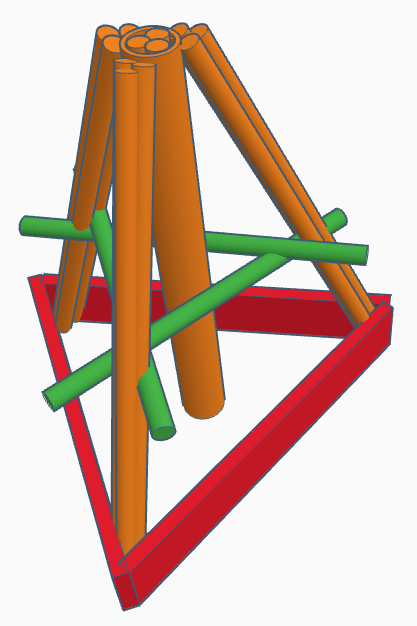
\includegraphics[width=0.5\linewidth]{model-overview}
		\caption{Overview of the model. The major members are shown in orange, the
			supporting members are shown in green, and the restraining piece is shown in red.}
		\label{fig:model-overview}
	\end{figure}

\subsection{Major Members}

The major members are one straight column erected vertically from the ground, and three
	slanted columns connecting the ground and the top of the vertical column. The points
	where the slanted columns contact the ground are the vertices of an equilateral triangle
	whose circumcenter is the point where the vertical column contacts the ground.

The major members are the longest members of the model and bear the most load. Therefore,
	they become unstable as the length increases as shown in Equation \ref{eq:eulers-load}.

\subsubsection{Pipe Configuration}

To address this issue, the major members were fabricated by combining three densly rolled
	newspaper pipes (termed as the \textbf{tri-pipe configuration}, Figure
	\ref{fig:tri-pipe-cross-section}) as opposed to using
	a single pipe (termed as the \textbf{mono-pipe configuration}, Figure
	\ref{fig:mono-pipe-cross-section}). It is easy to proove
	that the tri-pipe configuration is more effective than the mono-pipe configuration.

\begin{figure}[hbt]
	\centering
	\begin{subfigure}{0.3\linewidth}
		\centering
		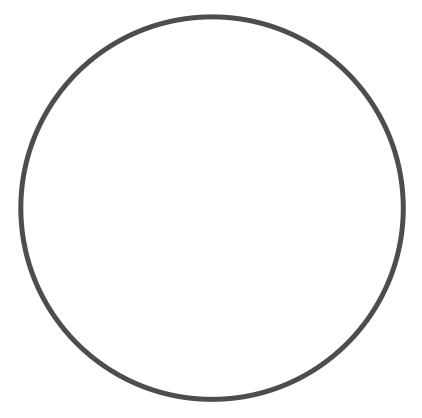
\includegraphics[width=\textwidth]{mono-pipe-cross-section}
		\caption{Mono-pipe configuration}
		\label{fig:mono-pipe-cross-section}
	\end{subfigure}
	\hspace*{0.1\linewidth}
	\begin{subfigure}{0.3\linewidth}
		\centering
		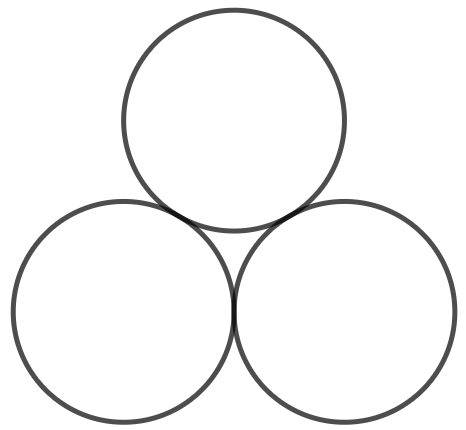
\includegraphics[width=\textwidth]{tri-pipe-cross-section}
		\caption{Tri-pipe configuration}
		\label{fig:tri-pipe-cross-section}
	\end{subfigure}
	\caption{Cross-sectional view of the mono-pipe configuration and the tri-pipe
		configuration.}
\end{figure}

Assume that both configurations have the same cross-sectional area $A$, and that the members
	are solid cylinders, each pipe of the tri-pipe configuration has a diameter $d$ and the
	pipe of the mono-pipe configuration has a diameter $D$. We can express $D$ in terms of $d$
	as $D = \sqrt{3}d$.

By calculation, we obtain the moment of inertia $I$ of both configurations as
	$I_{\text{tri}} = \frac{19}{64}\pi d^4 > I_{\text{mono}} = \frac{9}{64}\pi d^4$
	\cite{Riley:2007-Mechanics}.
	By adopting the tri-pipe configuration, the moment of inertia is increased by
	approximately $111\%$, which is a significant improvement.
	This shows that the tri-pipe configuration has a larger critical load.

Furthermore, by using Equation \ref{eq:radius-of-gyration}, we obtain the radii of gyration:
	$k_{\text{tri}} = \frac{\sqrt{57}}{12}d > k_{\text{mono}} = \frac{\sqrt{3}}{4}d$.
	$k_{\text{tri}}$ is approximately $45\%$ larger than $k_{\text{mono}}$.
	This shows that the tri-pipe configuration is more resistant to buckling and compressive
	stress.

\subsubsection{Paper-to-Paper Connection Structure}

After measurement, it was found that the longest side of one piece of newspaper is
	approximately $600$ mm. It is therefore impossible to fabricate a pipe with one single
	continuous piece of paper, and joining two pieces of paper is inevitable.

Two solutions were proposed to join pieces of paper for extending the length:
	\begin{enumerate}[noitemsep]
		\item By \textbf{overlapping} pieces of newspapers alternatively; or
		\item By placing two pieces of newspapers \textbf{side-by-side} and fixing them
			together with adhesive tape.
	\end{enumerate}

By comparison as illustrated in Table \ref{tab:connection-methods-comparison}, the overlapping
	method was chosen to form the pipes as it is more performant on the assessed aspects.

\begin{table*}[hbt]
	\caption{Compaison of the overlapping and side-by-side connection methods.}
	\centering
	\begin{tabular}{rll}
		\toprule
		Aspect & \textbf{Overlapping} & \textbf{Side-by-side} \\
		\midrule
		Load Distribution & Across all layers via friction and interlocking & Concentrated at the joint \\
		Strength & $\propto$ number of layers $\times$ strength of one layer & $\propto$ adhesive shear strength \\
		Stiffness & High due to composite action & Low due to tape not structurally integrated \\
		\bottomrule
	\end{tabular}
	\label{tab:connection-methods-comparison}
\end{table*}

\subsection{Supporting Members}
\label{sec:supporting-members}

The supporting members connect the adjacent slanted major members. They are supposed to
	hold major members in place through the tensile force generated by the strong and long
	paper fibres.

Since they do not bear compressive load but only tensile load, buckling was not a concern.
	Therefore, the supporting members were simply made of a single pipe.

\subsection{Restraining Piece}

Since the major members are slanted, it was projected that the vertical compressive load
	would decompose into downward vertical component and horizontal component directed
	away from the centre at the end of the slanted members. When the horizontal component
	is larger than the friction between the major members and the ground, the members would
	start to slide away from the centre, which would lead to most of the load being
	redistributed to the central member.

To restrain the horizontal movements of the members, the group has designed a restraining
	piece. The piece was made of several layers of continuous newspapers folded into a
	belt-like shape, which was then wrapped around the base.

Due to its continuous nature, the full potential of the paper fibres could be utilised
	to provide tensile strength. It was expected that when the members start to slide,
	the restraining piece would be able to counteract with its tensile strength.

\section{First Trial}

\begin{figure*}[hbt]
	\centering
	\begin{subfigure}{0.4\linewidth}
		\centering
		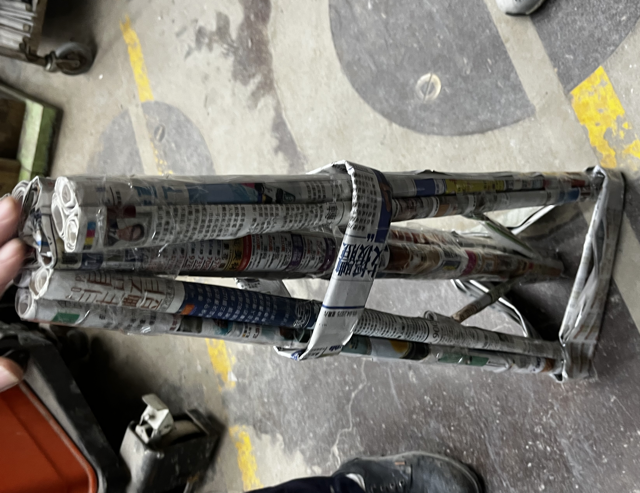
\includegraphics[width=0.85\linewidth, angle=270]{first-model-before-trial}
		\caption{Before}
		\label{fig:first-model-before-trial}
	\end{subfigure}
	\hspace*{0.05\linewidth}
	\begin{subfigure}{0.4\linewidth}
		\centering
		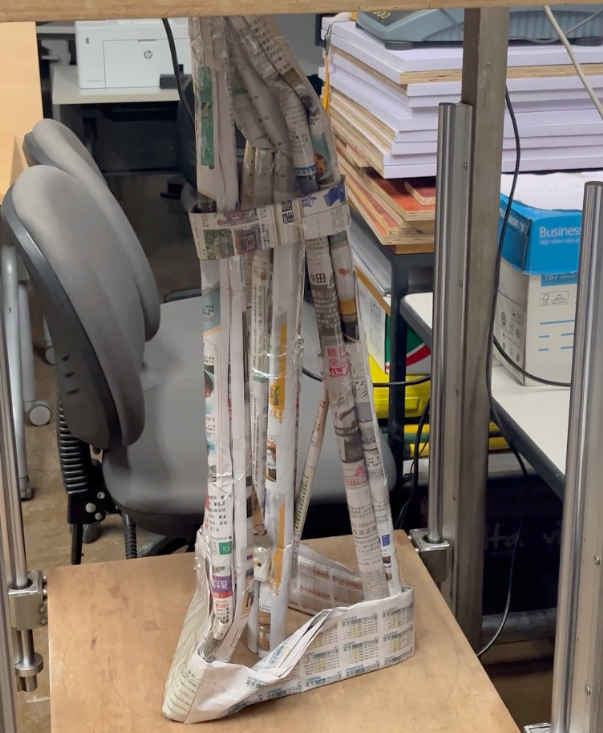
\includegraphics[width=0.7\linewidth]{first-model-after-trial}
		\caption{Immediately after failure}
		\label{fig:first-model-after-trial}
	\end{subfigure}
	\caption{The model before and after the first trial.}
\end{figure*}

\begin{figure*}[hbt!]
	\centering
	\begin{subfigure}{0.4\linewidth}
		\centering
		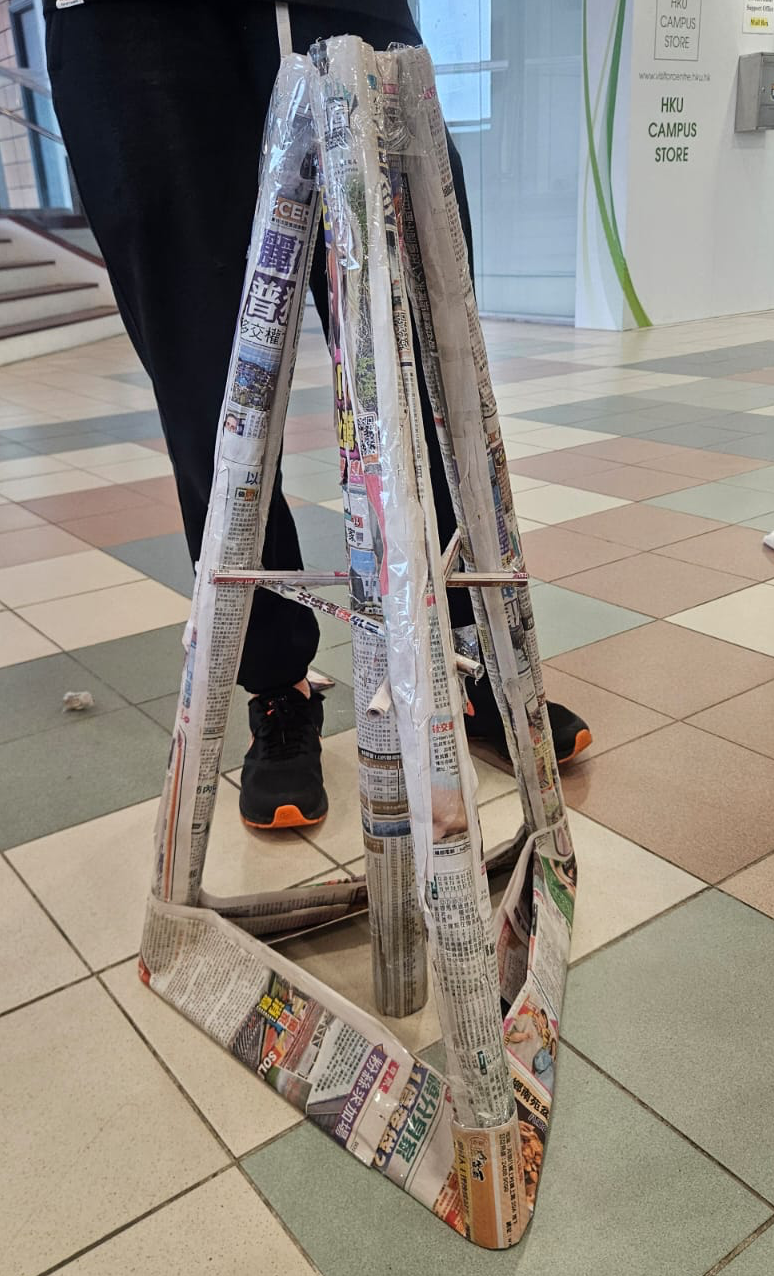
\includegraphics[width=0.5\linewidth]{final-model-before-trial}
		\caption{Before}
		\label{fig:final-model-before-trial}
	\end{subfigure}
	\begin{subfigure}{0.4\linewidth}
		\centering
		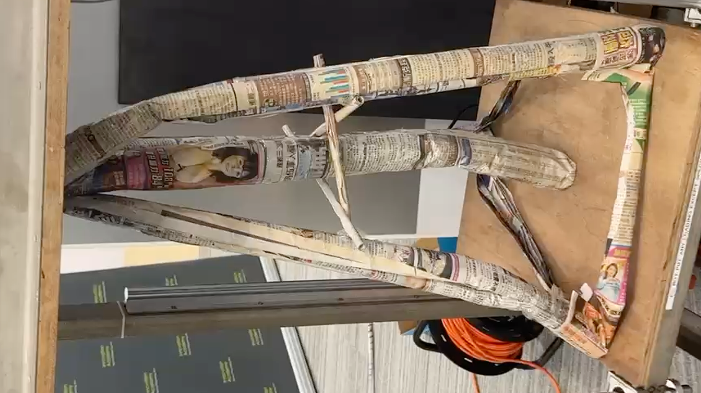
\includegraphics[width=0.8\linewidth, angle=270]{final-model-after-trial}
		\caption{Immediately after failure}
		\label{fig:final-model-after-trial}
	\end{subfigure}
	\caption{The model before and after the final trial.}
\end{figure*}

The model for the first trial was built with the following specifications:
\begin{enumerate}[noitemsep]
	\item \textbf{Weight and Height}: Within the limits.
	\begin{CJK*}{UTF8}{bsmi}
	\item \textbf{Newspaper Used}: Mainly the \textit{Sing Tao Daily} (星島日報).
	\end{CJK*}
	\item \textbf{Adhesive Tape Used}: Scotch Magic Tape (3M).
	\item \textbf{Design}: The supporting members did not observe the design as described
		in section \ref{sec:supporting-members}. However, those members did not have
		significant impact on the analysis of the model.
\end{enumerate}

The model is shown in Figure \ref{fig:first-model-before-trial}.

\subsection{Results}

The first model failed to withstand a minimum load of $500\text{ N}$. The model was
	able to withstand a load of $480\text{ N}$ before deformation occurred.
	It was observed that buckling occurred at the major members at a short instant
	after the load was applied (as shown in Figure \ref{fig:first-model-after-trial}).
	Of all the members, the three external slanted members were the first to buckle,
	while the central vertical member experienced the most deformation.

\subsection{Rationale of Failure}

After inspection of the failed model, the group has identified three major reasons
	that contributed to the failure of the model.

\subsubsection{Low Density of the Major Members}

All of the major members in the model were fabricated without aid of any tools. The
	newspaper pipes were rolled by hand, leaving large gaps between the layers of
	newspapers. This resulted in a low density of the major members.

To quantitatively analyse this issue, the gap-interleaving members can
	be approximated as a hollow cylinder of inner radius $r$ and outer radius $R$ and
	compared with a solid cylinder of radius $R$.
	The moments of inertia of the two models are
	$I_\text{hollow} = \frac{\pi}{64}(D^4 - d^4)$ and $I_\text{solid} = \frac{\pi}{4}D^4$.
	It is trivial to see that $I_\text{hollow} < I_\text{solid}$.
	By Equation \ref{eq:eulers-load}, the critical load of the hollow cylinder is
	less than that of the solid cylinder. This shows that the hollow cylinder is more
	prone to buckling.

Furthermore, during fabrication, the newspapers might have been rolled unevenly, resulting
	in folds and wrinkles on the surface of the pipes. This further reduce the stability of
	the major members.

\subsubsection{Presence of Weak Points at Paper-to-Tape Junctions}

While applying the adhesive tape on the pipes, the surfaces of the pipes were not
	thoroughly covered, resulting in surfaces that were exposed to air. This led to
	inconsistent surface stiffness as surfaces with adhesive tapes are stiffer than
	those without. When under compressive pressure, the joints at which surfaces with
	discontinuous stiffness meet are prone to buckling.

\subsubsection{Imbalance of Load Distribution Due to Mismatched Lengths of the Slanted Members}

The group was not rigorous in measuring the lengths of the slanted members. Prior to the
	first trial, the group has noticed that the structure was unable to support itself
	evenly on all columns, and that one of the slanted members remained not in contact with
	the ground. This resulted in an imbalance of load distribution. During compression,
	the stress was concentrated on the central member and the slanted members that were in
	contact with the ground, while the remaining member acted as a Zero Force Member.
	As a result, some of the members were subjected to stress that exceeded the designed
	limit and buckled, which is consistent with the observation.

\subsection{Measures Taken for Improvement}

In order to address the issues identified in the first trial, the group has taken
	the following measures to improve the model in fabrication of the model for the
	final trial.

\subsubsection{Rolling the Members with Tools to Increase Density and Avoid Defects}

The group has used thin cylindrical wooden rods to assist in rolling the newspapers into
	pipes. The rods were placed on the newspapers while rolling, such that the newspapers
	could bind tightly and uniformly, reducing gaps between layers and wrinkles on the surface.
	The rod was then removed after the pipe was rolled. This method streamlined pipe
	production and improved the strength of the major members.

\subsubsection{Apply Adhesive Tapes Thoroughly and Effectively}

The group has carefully applied the adhesive tapes on the pipes to ensure that the
	entire surface of the pipes were covered evenly with tapes. This is projected to
	increase the stiffness and uniformity of the surfaces.

In addition, the group has also applied more tapes at the top and bottom of the pipes
	as these are the areas that are subjected to the most stress and need to be reinforced.
	
\section{Final Trial}

The model for the final trial was built with the same specifications as the first trial,
	except that the design of the supporting members was changed to observe the design as
	described in section \ref{sec:supporting-members}. The model is shown in Figure
	\ref{fig:final-model-before-trial}.

\subsection{Results}

In the final trial, the model was able to withstand a load of $767\text{ N}$, which satisfied
	the requirement of the practical work and was a significant improvement from the first
	trial.

As opposed to the first trial, buckling occurred almost simultaneously at all members when
	the critical load was approached. This displayed that the load was distributed uniformly
	throughout the model, showing that the alterations made to the design was effective.

\subsection{Reflection and Possible Improvements}

Despite the success of the final trial, the group has identified possibility for further
	improvements.

From the deformed model, it was observed that buckling started but did not progress
	significantly until the supporting members dislocated from the major members.
	It has shown that the supporting members were indeed effective in providing stability
	and the reinforcement of which could have further increased the critical load.

Additionally, the group has observed that the restraining piece that was expected to restrain
	horizontal movements of the major members almost bore no load during both trials.
	This has shown that the group has overestimated the magnitude of the horizontal
	movements and underestimated the friction between the major members and the ground.
	Much of the weight could have been saved or diverted to other components of the model
	if the restraining piece was not used.

\section{Conclusion}

This practical work has encouraged the group to consolidate and apply the knowledge
	learned in class, and to explore further beyond the scope of the course.
	THe group has gained a deeper understanding of the principles and theorems in
	the field of structural and material mechanics. The group has also earned precious
	experience through the process of designing, trial-and-error, observing, and reflecting.
	The practical work has also offered an opportunity for the group to communicate
	effectively.

\phantomsection
\section*{Acknowledgments} % The \section*{} command stops section numbering
\addcontentsline{toc}{section}{Acknowledgments} % Adds this section to the table of contents

We would like to express our profound gratitude to the course instructors
	and teaching assistants for providing guidance and support upon consultation.

We would also like to thank all the members of Group C9 for their efforts and
	contribution to the practical work.

We would like to thank the library of the University of Hong Kong for providing an
	extensive collection of materials for reference and research.

Finally, we would like to thank the authors Mathias Legrand and Vel for providing this
	professional \LaTeX\,template.

%----------------------------------------------------------------------------------------
%	REFERENCE LIST
%----------------------------------------------------------------------------------------

\phantomsection
\bibliographystyle{unsrt}
\bibliography{references.bib}

%----------------------------------------------------------------------------------------

\end{document}